\documentclass[10pt, conference]{IEEEtran}
\usepackage[english]{babel}
\usepackage[usenames]{color}
\usepackage{colortbl}
\usepackage{comment}
\usepackage{graphicx}
\usepackage{epsfig}
\usepackage{array, colortbl}
\usepackage{listings}
\usepackage{epstopdf}
\usepackage{multirow}
\usepackage{rotating}
%\usepackage{subfigure}
%\usepackage{subfig}
\usepackage{float}
\usepackage[obeyspaces,hyphens,spaces]{url}
\usepackage{balance}
\usepackage{fancybox}
\usepackage{scalefnt}
\usepackage[normalem]{ulem}
%\pagestyle{plain}
\pagenumbering{arabic}
\pagestyle{empty}
\clubpenalty = 10000
\widowpenalty = 10000
\displaywidowpenalty = 10000
\usepackage{cleveref}
\usepackage{latexsym}
\usepackage{amsfonts}
\usepackage{amssymb}

\usepackage{graphicx}
\usepackage{caption}
\usepackage{subcaption}


\makeatletter
\renewcommand{\paragraph}[1]{\noindent\textsf{#1}.}

\title{Cloud Computing Performances on Amazon EC2 Instances}
\author{Zeinab Kermansaravi, Mohammed Sayagh
    \\
    \emph{azadeh.kermansaravi, mohammed.sayagh}@polymtl.ca}

\begin{document}
\maketitle

\begin{abstract}
One of the most important challenges to migrate software application to Cloud is to choose the right instance type, which gives the right resources to our application. Our analysis based upon five benchmarks on five Cloud instances provides a difference of performance, helping users to choose the right instance for their applications. 
\end{abstract}

\section{Introduction}
\label{sec:introduction}


\indent Cloud computing is a general term for the delivery of hosted services over the Internet. It means that instead of all the computer hardware and software you're using sitting on your desktop, or somewhere inside your company's network, it's provided for you as a service by another company and accessed over the Internet, usually in a completely seamless way. It is just somewhere up in the nebulous "cloud" that the Internet represents. Cloud computing is a word that means different things to different people which promises several attractive benefits for businesses and end users such as Self-service provisioning, Elasticity and Pay per use.\\
\indent Nowadays, “Cloud Computing” is most discussed term in business and academic environment. Because of the increasing popularity, many giant IT companies such as Microsoft, IBM, Google and Amazon interest Cloud Computing. Many managers in small business and academicians in universities are not aware of benefits and characteristic of minimizing the cost of cloud computing. IT companies are eager to encourage educational adoption of cloud computing; for example, Google has designed cloud based GoogleApps for educational usage, and another example, IBM launched IBM Cloud Academy that provides a global forum for educators, researchers and IT professionals from education industry to pursue cloud computing initiatives, develop skills and share best practices to reduce operating costs while improving quality and access to education.\\
\indent Due to significant and daily increase in cloud computing development, some important challenges in the field are as follows: Optimized server utilization, Cost saving, Dynamic scalability, Shortening development life cycle, Reducing time for implementation, Data location, Cloud security policy/procedures transparency and Disaster recovery.\\
\indent In this regard, we perform a through analysis to propose which instance could be used for associated application.

\section{Background}
\label{sec:backgr-relat-work}

\subsection{Instances}
\begin{table*}
\begin{center}
\begin{tabular}{|l|l| }
  \hline
  Instance Family & Current Generation Instance Types \\
  \hline
  General Purpose & t2.micro, t2.small, t2.medium,  m3.medium, m3.large, m3.xlarge, m3.2xlarge \\
  Compute optimized &  c4.large, c4.xlarge, c4.2xlarge, c4.4xlarge, c4.8xlarge, c3.large,  c3.xlarge, c3.2xlarge, c3.4xlarge, c3.8xlarge\\
  Memory optimized & r3.large, r3.xlarge, r3.2xlarge, r3.4xlarge, r3.8xlarge \\
  Storage optimized & i2.xlarge, i2.2xlarge, i2.4xlarge, i2.8xlarge, hs1.8xlarge \\
  GPU instances & g2.2xlarge \\
  \hline
\end{tabular}
\caption{\label{table:instancess} Current Generation Instances}
\end{center}
\end{table*}


We have used five different instances in our case study based on Ubuntu includes t2.micro, t2.small, t2.medium, c3.large and c3.xlarge. When you launch an instance, the instance type that you specify determines the hardware of the host computer used for your instance. Each instance type offers different compute, memory, and storage capabilities. Amazon EC2 provides each instance with a consistent and predictable amount of CPU capacity, regardless of its underlying hardware. Amazon EC2 provides the current and previous generation instance types listed in the table \ref{table:instancess}.  

T2 instances are designed to provide moderate baseline performance and the capability to burst to significantly higher performance as required by your workload. They are intended for workloads that don't use the full CPU often or consistently, but occasionally need to burst. 
Each T2 instance receives CP Credits continuously at a set rate depending on the instance size.  The t2.micro and t2.small instance types launch with an initial balance of 30 CPU credits, and the t2.medium instance type launches with 60 CPU credits. This initial credit balance is designed to provide a good startup experience. The maximum credit balance for an instance is equal to the number of CPU credits received per hour times 24 hours. For example, a t2.micro instance earns 6 CPU credits per hour and can accumulate a maximum CPU credit balance of 144 CPU credits
T2 instances are well suited for general purpose workloads, such as web servers, developer environments, and small databases. T2 instances are currently available in three instance sizes: t2.micro, t2.small, and t2.medium. Customers can launch T2 instances using the AWS management console, Amazon EC2 command line interface, and the AWS SDKs. 

Features:

\begin{itemize}

\item High Frequency Intel Xeon Processors operating at 2.5GHz with Turbo up to 3.3GHz
\item Burstable CPU, governed by CPU Credits, and consistent baseline performance
\item Lowest-cost general purpose instance type, and Free Tier eligible (t2.micro only)
\item Balance of compute, memory, and network resources

\end{itemize}

Use Cases: Development environments, build servers, code repositories, low-traffic web applications, early product experiments, small databases.  

The C3 instance types deliver their highest processor performance in Amazon's cloud. The C3 instances are backed by Intel Xeon E5 "Ivy Bridge" processors, use SSD-based storage, support AVX and Turbo as part of the Ivy Bridge feature set, and also deliver on improved network performance in the cloud. Amazon also announced new I/O-focused instance types last week too, but of most interest to us at Phoronix are the C3 instance types for compute-intensive workloads. Over the conventional C1 instances, the C3 instances use the faster Intel Ivy Bridge processors and double the memory per vCPU and use solid-state storage. 
Features:
\begin{itemize}

\item High Frequency Intel Xeon E5-2680 v2 (Ivy Bridge) Processors
\item Support for Enhanced Networking
\item Support for clustering
\item SSD-backed instance storage

\end{itemize}
Use Cases: High performance front-end fleets, web-servers, batch processing, distributed analytics, high performance science and engineering applications, ad serving, MMO gaming, video-encoding, and distributed analytics \cite{ref1} \cite{ref2}. 


Table \ref{table:instancess} provides their differences, besides, Table \ref{table:price} shows the difference between the price of each instance type \cite{ref3} \cite{ref4}. 

\begin{table*}
\begin{center}
\begin{tabular}{|l|l|l|l|l|l|l|l|l|l|}
  \hline
  API Name & Memory & Compute Unite & Cores & Storage & Arch & I/O Performance & Linux cost & Windows cost \\
  \hline
  t2.micro & 1.0 GB & 1 units(Burstable) & 1 cors & 0GB (EBS only) & 32/64-bit & Low to Moderate & \$0.013 h* & \$0.018 h\\
  t2.small & 2.0 GB & 1 units(Burstable) & 1 cors & 0GB (EBS only) & 32/64-bit & Low to Moderate & \$0.026 h & \$0.036 h\\
  t2.medium & 4.0 GB & 2 units(Burstable) & 2 cors & 0GB (EBS only) & 64-bit & Low to Moderate & \$0.052 h & \$0.072 h\\
  c3.large & 3.75 GB & 7 units & 2 cors & 32GB (SSD) & 64-bit & Moderate & \$0.105 h& \$0.188 h\\
  c3.xlarge & 7.5 GB & 14 units & 4 cors & 80GB (SSD) & 64-bit & Moderate/500Mbps & \$0.210 h & \$0.376 h\\
   \hline
\end{tabular}
\caption{\label{table:price} compare EC2 instances using Amazon's instance type and pricing pages, *per hour}
\end{center}
\end{table*}





\subsection{Benchmarks}

In this section, we provide the Benchmarks used in our analyzes. We have used \textit{UnixBench} to analyze the CPU performance, \textit{dd if=/dev/zero of=sb-io-test bs=1M count=1k conv=fdatasync} to analyze the IO, ioping to analyze IOPS, Redis to analyze the memory performance, and Dbench to analyze Disk and Network Throughput performances. 

\subsubsection{UnixBench}


UnixBench is a benchmark used to evaluate the general performances of a server, specially it is used to measure the CPU. It runs the following tests:

\begin{itemize}

\item Dhrystone: This test focus on the operations on the strings.
\item Whetstone: This test focus on the operations on the floats.
\item Execl Throughput: This test aims at measuring the number of call \textit{execl} that could be done by second.
\item Pipe Throughput: This test aims at evaluating the pipes' bandwidth, a process read or write on a pipe.
\item Pipe-based Context Switching: This test aims at measuring the communication between process.
\item Process Creation: This test aims at measuring the creation of a process
\item Shell Scripts: It represents the execution time of a script by simulating the common operations. 

\end{itemize}

\subsubsection{dd if=/dev/zero of=sb-io-test bs=1M count=1k conv=fdatasync}

This benchmark is used to compute the performance of reading/writing on a disc, bellow this command : \textit{dd if=/dev/zero of=sb-io-test bs=1M count=1k conv=fdatasync}. The command \textit{dd} is used to copy a file by the selection of just a part of the file. The parameters of this command are:

\begin{itemize}

\item if: What we should write, in our example, we write NULL (/dev/zero).
\item of: The file name where the command \textit{dd} writes.
\item bs: The size of block to write.
\item count: The count of blocks to write. 
\item conv: The conversion to do. For example: \textit{conv=lcase} will convert the character to lower case characters.

\end{itemize}

Therefore, the command \textit{dd if=/dev/zero of=sb-io-test bs=1M count=1k conv=fdatasync} is used to evaluate the performance of Disk IO. It will copy in the file \textit{sb-io-tests}, 1M x 1k NULL (/dev/zero).

It gives as results, the record-in, record-out, the size copied, the time spent to copy data, and the copy speed.

\subsubsection{ioping}

By the same principle of the command \textit{ping}, which evaluate the network latency, we have the command \textit{ioping} used to measure the monitor I/O latency. However, it does many request, we can limit the number of request by the parameter \textit{-c number\_of\_requests}. It gives as results the minimum, the average, the maximum time of all requests done.

\subsubsection{Redis}

\indent Redis is an open source, in-memory advanced key-value store with optional persistence to disk. Redis command line interface ${redis-cli}$ is used to analyze the Redis metrics and access the actual data. Redis includes the redis-benchmark utility which is used to evaluate the performance of memory using simulates running commands done by $N$ clients at the same time sending $M$ total queries. Basic syntax of redis benchmark is shown below:\\

\indent redis-benchmark [option] [option value]\\

\indent When Redis-benchmark is run, lots of tet with specific definitions are done as following:

\begin{itemize}

\item PING-INLINE and PING-BULK: This command is often used to test if a connection is still alive, or to measure latency.
\item SET: It Set key to hold the string value. If key already holds a value, it is overwritten, regardless of its type. Any previous time to live associated with the key is discarded on successful SET operation.
\item GET: It Get the value of key. If the key does not exist the special value nil is returned. An error is returned if the value stored at key is not a string, because GET only handles string values.
\item INCR: This comment increments the number stored at key by one. If the key does not exist, it is set to 0 before performing the operation. An error is returned if the key contains a value of the wrong type or contains a string that can not be represented as integer. This operation is limited to 64 bit signed integers.
\item LPUSH: This comment insert all the specified values at the head of the list stored at key. If key does not exist, it is created as empty list before performing the push operations. When key holds a value that is not a list, an error is returned.
It is possible to push multiple elements using a single command call just specifying multiple arguments at the end of the command. Elements are inserted one after the other to the head of the list, from the leftmost element to the rightmost element.
\item LPOP: It removes and returns the first element of the list stored at key.
\item SADD: Add the specified members to the set stored at key. Specified members that are already a member of this set are ignored. If key does not exist, a new set is created before adding the specified members. An error is returned when the value stored at key is not a set.
\item SPOP:This command removes and returns a random element from the set value stored at key.
\item LRANGE: Returns the specified elements of the list stored at key. The offsets start and stop are zero-based indexes, with 0 being the first element of the list (the head of the list), 1 being the next element and so on. These offsets can also be negative numbers indicating offsets starting at the end of the list. For example, -1 is the last element of the list, -2 the penultimate, and so on. Note that if you have a list of numbers from 0 to 100, LRANGE list 0 10 will return 11 elements, that is, the rightmost item is included.
\item MSET:  MSET replaces existing values with new values, just as regular SET. See MSETNX if you don't want to overwrite existing values. MSET is atomic, so all given keys are set at once. It is not possible for clients to see that some of the keys were updated while others are unchanged.
\end{itemize}


\subsubsection{Dbench}
\indent Dbench is a Filesystem benchmark which generates load patterns, but without requiring a lab of Windows load generators to run. It is used to calculate the performance of Disk and Network Troughput. Dbench is a utility to benchmark a system based on client workload profiles.\\
\indent Dbench takes only one parameter on the command line, which is the number of processes (clients) to start. Issuing the command “dbench 30” for example, creates 30 parallel processes of dbench. All processes are started at the same time and each of them runs the same workload. The workload for each dbench process is specified by a client.txt configuration file in the working (testing) directory. It consists of a mixture of file system operations executed by each dbench process. dbench runs with n parallel processes and delivers only one value as a result. The resulting value is an average throughput of the file system operations described in client.txt and measured in megabytes per second.\\
\indent It can also take the following options:\\

\begin{itemize}
\item -c client.txt : Use this as the full path name of the client.txt file (the default is $/usr/share/dbench/client.txt$).
\item -s: Use synchronous file IO on all file operations.
\item -t TIME: set the runtime of the benchmark in seconds (default 600)
\item -D DIR: set the base directory to run the filesystem operations in
\item -x: enable xattr support, simulating the xattr operations Samba4 would need to perform to run the load
\item -S: Use synchronous IO for all directory operations (unlink, rmdir, mkdir and rename). The tbench program takes a number, which indicates the number of clients to run simultaneously,  and a server name: $tbench_srv$ should be invoked on that server before invoking tbench. tbench can also take the following options:
\item -c loadfile: Use this as the full path name of the client.txt file (the default is $/usr/share/dbench/client.txt$).
\item -T option[,...]: This sets the socket options for the connection to the server. 
\end{itemize}

\indent dbench allows you to get a feel for how well the file system on a CIFS server will perform when presented with the NetBench workload. The Common Internet File System (CIFS) is a file sharing protocol. Client systems use this protocol to request file access services from server systems over a network. It is based on the Server Message Block protocol widely in use by personal computers and workstations running a wide variety of operating systems. \\
\indent There are two benchmark description files. One called $client-plain.txt$, the other called $client-oplocks.txt$.  Each of these consists of a series of lines, one for each operation that the file describes. Each operation contains information about all the relevant parameters needed by each operation. Both files contain only the following 13 operations.\\

\indent Close\\
\indent Deltree\\
\indent Flush\\
\indent NTCreateX\\
\indent QUERY FILE INFORMATION\\
\indent QUERY FS INFORMATION\\
\indent QUERY PATH INFORMATION\\
\indent ReadX\\
\indent Rename\\
\indent mkdir\\
\indent Unlink\\
\indent WriteX\\
\indent ...\\

\indent This is a relatively small number of operations. There are no Oplock specific operations in the mix because the Netbench benchmark only causes self-breaks, which are all handled transparently by libsmb. It is clear that with oplocks enabled on the server, many fewer operations result, and the client is able to satisfy many requests from the local cache.\\
\indent The format of each line is relatively simple. The following is an example: 

\begin{figure}[h!]
	\centering
	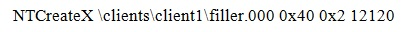
\includegraphics[width=7cm]{figure1.jpg}
\end{figure} 

\indent This specifies that the CIFS op to be made is an NTCreateX request. The following table summarizes the occurrence of each operation within each benchmark trace:
\begin{figure}[h!]
	\centering
	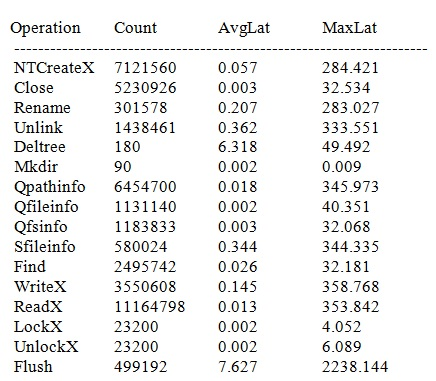
\includegraphics[width=8cm]{figure2.jpg}
\end{figure} 

\begin{itemize}
\item  NTCreateX, Qpathinfo (QueryPathInfo), Qfileinfo (QueryFileInfo), Sfileinfo(SetPathInfo) are  kind of a file create operations. 
\item ReadX, WriteX, Flush, close are the file operations which read the file, write on the file and close the file.
\item  Deltree is used to remove a directory with all of its subdirectories and files, uses the deltree EXEC command. 
\item Mkdir is used to create a directory. 
\item Rename operation, renames a file on a WAAS device.
\item When a file is created, it is given a link count of one. As you add and remove links to the file, this link count is incremented and decremented.  Unlink is used to remove the links.  
\end{itemize}

\indent The output is very simple: just a list of the MB/s achieved by the run.


\subsubsection{netpref}
\indent Netperf is a software application that provides network bandwidth testing between two hosts on a network. It supports Unix domain sockets, TCP, SCTP, DLPI and UDP via BSD Sockets. Netperf provides a number of predefined tests e.g. to measure bulk (unidirectional) data transfer or request response performance. Once built, two binaries (netserver and netperf) and a bunch of scripts are noted. The scripts are great for generating a whole suite of tests at once, and they also serve as good examples of some of the many command line arguments netperf takes. Visiting the remote system and starting up a netserver (daemon) on the considered port or some other make some results like Figure 1:\\

\$netserver\\
\indent Starting netserver at port 127.0.0.1\\

This daemon will typically run until killed (like the lmbench daemon, unlike the netpipe daemon). Multiple tests can be run to the target host once the daemon is running.

Then return to your source host and run netpipe as shown in Figure 1:
\begin{figure}[h!]
	\centering
	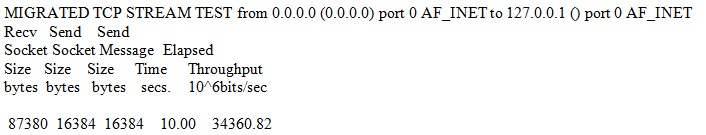
\includegraphics[width=10cm]{figure4.jpg}
\end{figure} 

This particular invocation says to test for 10 seconds continuously, sending a TCP stream of data to the target 127.0.0.1 with a message size of 16384 (recall, the largest message that will fit in an MTU) using a large send and receive buffer (87380, 16384) on both ends which results the troughput equal to 34360.82 bit/sec. Many other options are possible -- netperf is a powerful command with many distinct ways of running. 



\section{Approach}
\label{sec:approach}

In this section, we provide the approach used to extract data. While the first step consists of creating the instances, the second one consists of computing data. 

We have created the first instance of type \textit{t2.micro}, we have also created a script to compute data. Therefore, to create another instance, we have used the image of the first one. Hence, we have created the types of instances consisting of \textit{t2.small}, \textit{t2.medium}, \textit{c3.large}, and \textit{c3.xlarge}.

While each instance depends on where it is deployed, which could impact its performance, we have created five instances for each instance type. For example, we have created five instances for the instance type \textit{t2.micro}.


To compute data, we have used the benchmarks described above. Since the performance of Cloud instances change over time, because there are many instances deployed in the same infrastructure, we execute each benchmark five times.

While we have five instances type, 5 instances for each type, and five execution for each benchmark. The number of executions is 125.

To analyze the results, we have used boxplots to show the difference between instances. Moreover, to understand the results, we have used the detailed information of each benchmark output, and the characteristics of each instance type.

\section{Results}
\label{sec:results}

In this section, we provide the benchmarks results.

\subsection{CPU performances}

\textbf{Results. The averages of UnixBensh results for each instance are: 600.628 for the instance \textit{t2.micro}, 1482.136 for the instance \textit{t2.small}, 2705.132 for the instance \textit{t2.medium}, 2255.052 for the instance \textit{c3.large}, and 3282.676 for the instance \textit{c3.xlarge}}.

\begin{figure}
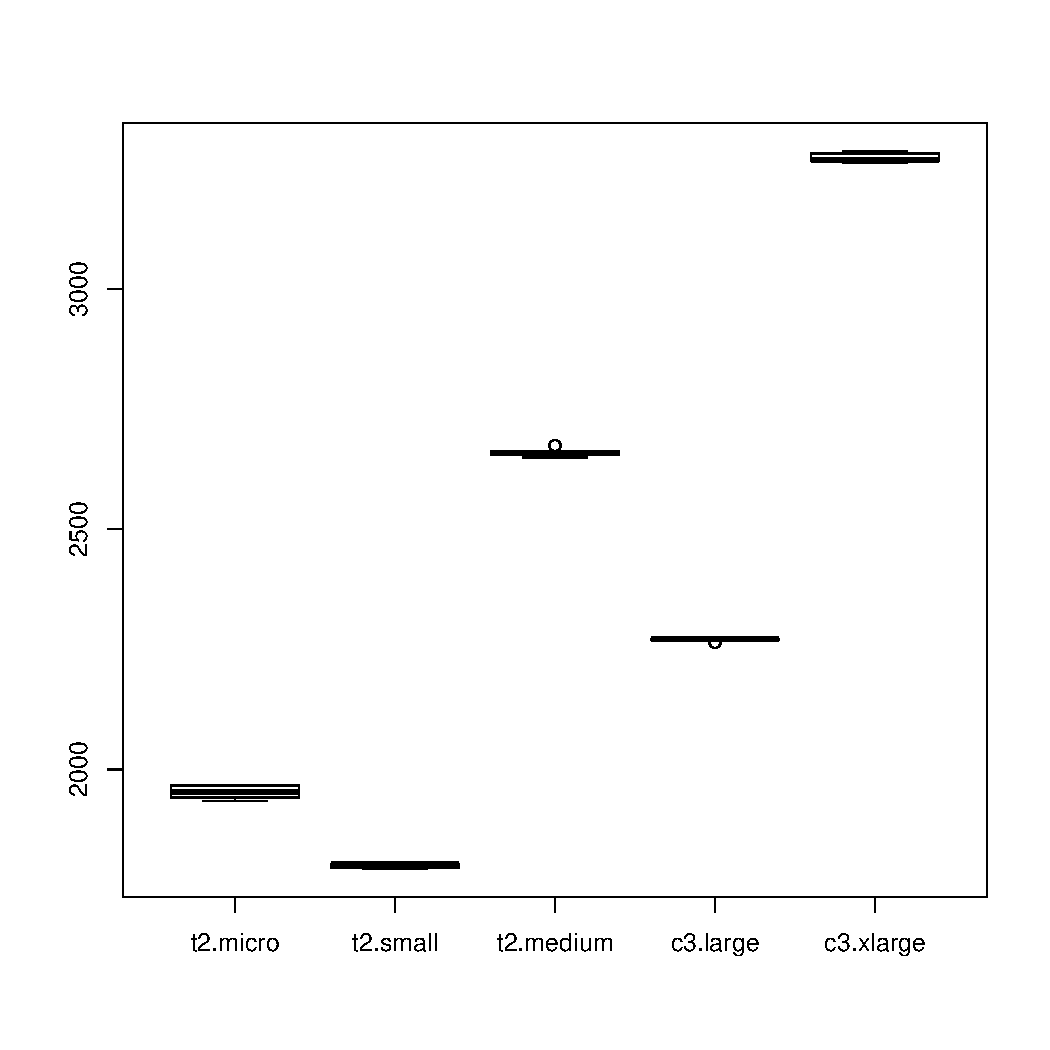
\includegraphics[width=0.5\textwidth]{plots/UnixBench.pdf}
\caption{CPU benchmark results}
\label{fig:UnixBenchResult}
\end{figure}

As highlighted by Figure \ref{fig:UnixBenchResult}. The minimum value of \textit{UnixBench} benchmark results for the instance \textit{t2.micro} is \textit{1933.5}, whereas the maximum is \textit{1967}. The minimum for the instance \textit{t2.small} is \textit{1793.6} and the maximum is \textit{1806.8}. \textit{t2.medium} provides as a minimum result of the same benchmark \textit{2649.2}, where the maximum is \textit{2674.1}. The minimum value of \textit{c3.large} is \textit{2264.2} where the maximum is \textit{2271.8}. \textit{c3.xlarge} provides a minimum of \textit{3263.1} and a maximum of \textit{c3.xlarge}.

The smallest value of \textit{UnixBench} benchmark is provided by the instance \textit{t2.small}, and the maximum is provided by the instance \textit{c3.xlarge}.

As provided by Figure \ref{fig:UnixBenchResult}, the order of instances by the \textit{UnixBench} benchmark is as follow: \textit{t2.micro, t2.small, c3.large, t2.medium, c3.xlarge}.

\textbf{Discussion}. We observe that we have three categories of instances in Figure \ref{fig:UnixBenchResult}. We can classify the instances in three main clusters. While the first one is represented by the instances \textit{t2.micro} and \textit{t2.small}, which have one virtual processor. The second category is presented by \textit{t2.medium} and \textit{c3.large}, which contains two virtual processor. The third category contains the instance \textit{c3.xlarge}, it contains 4 virtual CPU. Hence, the difference between the three category is due to the number of virtual processor.

Moreover, There is a difference between the instances \textit{t2.micro} and \textit{t2.small}. By analyzing the benchmark results, we have found that the main difference is in the test \textit{File Copy 4096 bufsize 8000 maxblocks}, which consists of copying a large size, which gives the important different score (around 5910.3 for the instance \textit{t2.micro} and 4998.4 for the instance \textit{t2.small}). 

The main difference between \textit{t2.medium} and \textit{c3.large} is principally due to the test \textit{Dhrystone 2 using register variables}, which tests the operations on the strings. Hence, \textit{t2.medium} has a better CPU performance than \textit{c3.large}, especially on the operations on the strings.


\

\noindent\fbox{%
    \parbox{8.5cm}{
	\textit{\newline
	The instance providing the highest CPU performance is \textit{c3.xlarge}.
	\\
	The instance providing the lowest CPU performance is \textit{t2.micro}.
\newline
	} 
    } \par
}

\

\

\subsection{IO performances}

\begin{figure}
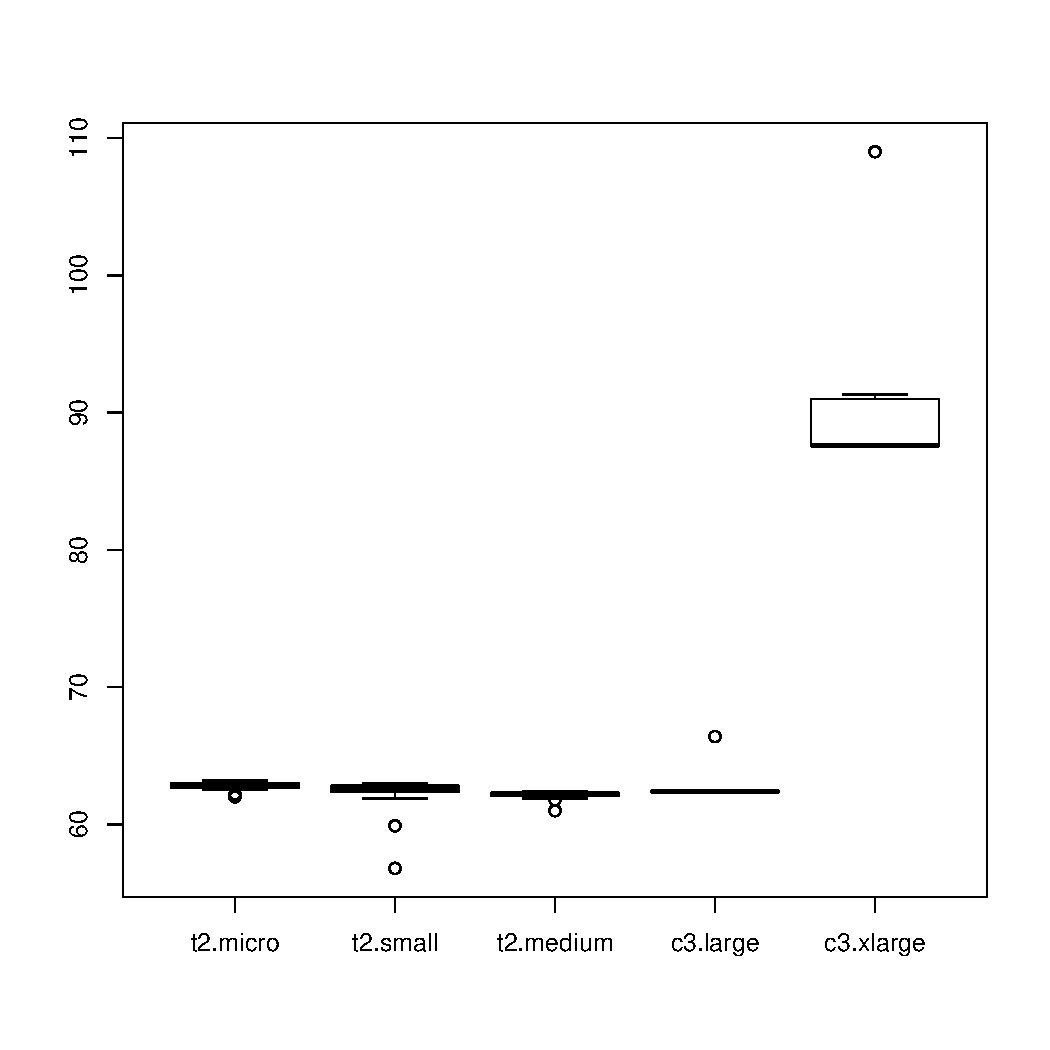
\includegraphics[width=0.5\textwidth]{plots/dd.pdf}
\caption{IO benchmark results}
\label{fig:ddResult}
\end{figure}

\textbf{Results. The averages of IO Benchmark results for each instance are: 62.812 for the instance \textit{t2.micro}, 62.308 for the instance \textit{t2.small}, 62.152 for the instance \textit{t2.medium}, 63.2 for the instance \textit{c3.large}, and 91.72 for the instance \textit{c3.xlarge}}

As highlighted by Figure \ref{fig:ddResult}. The minimum value of \textit{IO} benchmark results for the instance \textit{t2.micro} is \textit{62 MB/s}, whereas the maximum is \textit{63.2 MB/s}. The minimum for the instance \textit{t2.small} is \textit{56.8 MB/s} and the maximum is \textit{63 MB/s}. \textit{t2.medium} provides as a minimum result of the same benchmark \textit{61 MB/s}, where the maximum is \textit{62.4 MB/s}. The minimum value of \textit{c3.large} is \textit{62.4 MB/s} where the maximum is \textit{66.4 MB/s}. \textit{c3.xlarge} provides a minimum of \textit{87.5 MB/s} and a maximum of \textit{109 MB/s}.

The smallest value of \textit{IO} benchmark is provided by the instance \textit{t2.medium}, and the maximum is provided by the instance \textit{c3.xlarge}.

As provided by Figure \ref{fig:ddResult}, \textit{t2.micro, t2.small, t2.medium, and c3.large} have approximately the same median, whereas \textit{c3.xlarge} has the higher median.


\textbf{Discussion.} From the comparison provided in Figure \ref{fig:ddResult}, the instance \textit{c3.xlarge} has the highest speed of reading/Writing on disk. We refer these results to the I/O Performances, where the instance \textit{c3.xlarge} has "Moderate/500Mbps", and the other instances have "Low to moderate" or "Moderate".

\

\noindent\fbox{%
    \parbox{8.5cm}{
	\textit{\newline
	All the instances provide approximately the same IO performance, except the instance \textit{c3.xlarge}, which provide the highest IO performance.
\newline
	} 
    } \par
}

\

\

\subsection{IOPS performances}


\begin{figure}
	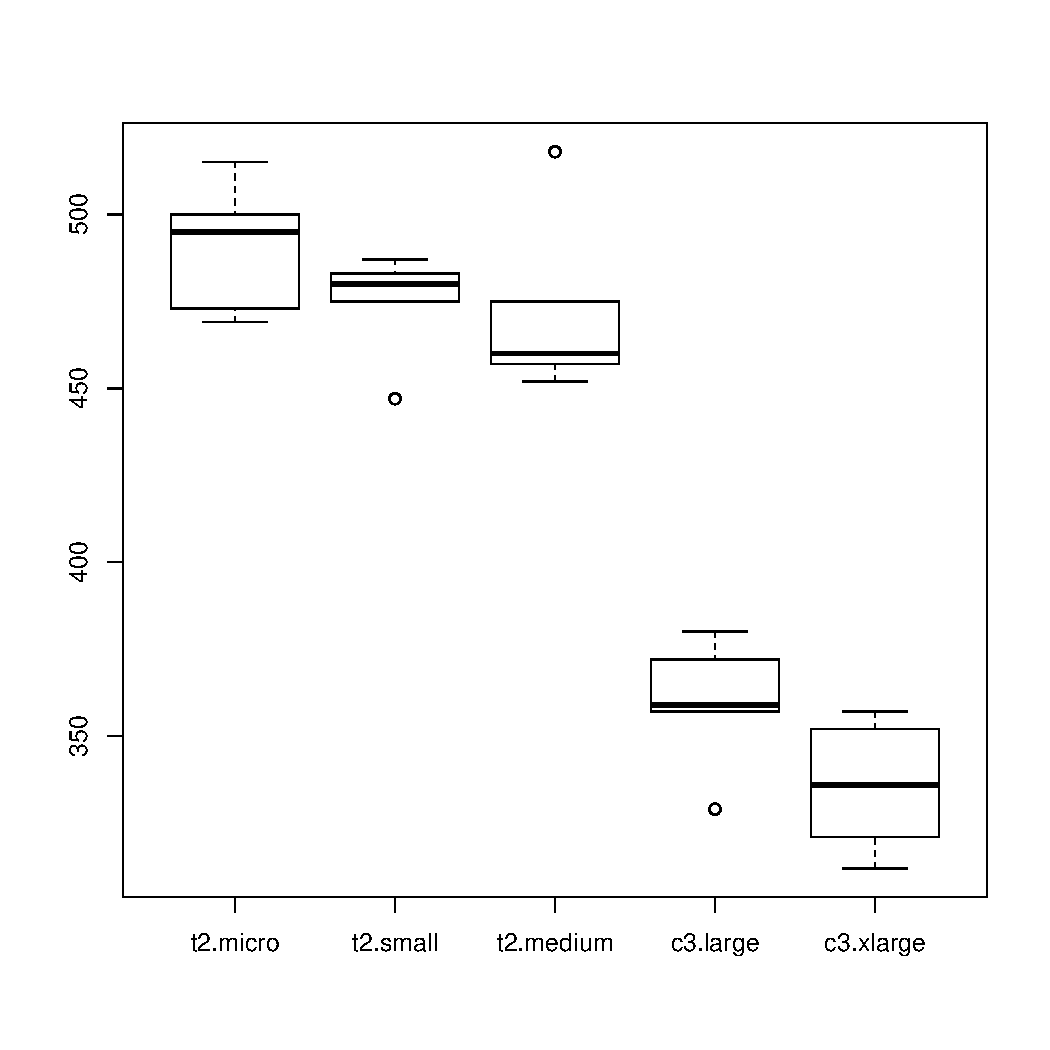
\includegraphics[width=0.5\textwidth]{plots/iopingAvr.pdf}
	\caption{\label{fig:IOPSResults} IOPS benchmark comparison of the average results (us)}
\end{figure}


\textbf{Results. The averages of IOPS Benchmark results for each instance are: 520.64 us for the instance \textit{t2.micro}, 468.96 us for the instance \textit{t2.small}, 464.64 us for the instance \textit{t2.medium}, 354.16 us for the instance \textit{c3.large}, and 355.84 us for the instance \textit{c3.xlarge}}.

As highlighted in Figure \ref{fig:IOPSResults}, the minimum time needed for the instance \textit{t2.micro} is 463 us, whereas the maximum is 712 us. 400 us is the minimum and 502 us is the maximum for the instance \textit{t2.small}, \textit{t2.medium} provides as minimum value 368 us and 553 us as maximum value, the minimum time needed for the instance \textit{c3.large} is 302 us and the maximum is 545 us. The minimum for the instance \textit{c3.xlarge} is 310 us and the maximum is 427 us. 

As provided in Figure \ref{fig:IOPSResults}, each instance has its own median time to provide an IOPS result, while the instance providing a minimum time is the better, and the one providing the higher one is the worse. The instances are ordered from the low performed to the high performed instance as follow: \textit{c3.xlarge, c3.large, t2.medium, t2.small, and t2.micro}.

\textbf{Discussion}. To understand the differences between the instances studied, we analyzed their storage differences. We can explain this difference, by the fact that the instance \textit{t2.micro, t2.small, and t2.medium} use only \textit{EBS} for the storage, which refers to shared disc with other machines, hence it accesses could be less performed because the same device is used by many other machines at the same time, where \textit{c3.large and c3.xlarge} use a dedicated storage device, which consists of 32 GB (2 * 16 GB SSD) for the instance \textit{c3.large} and 80 GB (2 * 40 GB SSD).

\

\noindent\fbox{%
    \parbox{8.5cm}{
	\textit{\newline
	The best instances providing the best IOPS performances are \textit{c3.large} and \textit{c3.xlarge}, while the lowest performance value is provided by the instance \textit{t2.micro}.
\newline
	} 
    } \par
}

\

\

\subsection{Disk performances}

\textbf{The averages of DBench results for each instance are: 227.66148 MB/sec for the instance \textit{t2.micro}, 229.51488 MB/sec for the instance \textit{t2.small}, 146.0973376 MB/sec for the instance \textit{t2.medium}, 280.305588 MB/sec for the instance \textit{c3.large}, and 332.16496 MB/sec for the instance \textit{c3.xlarge}}.


\begin{figure}
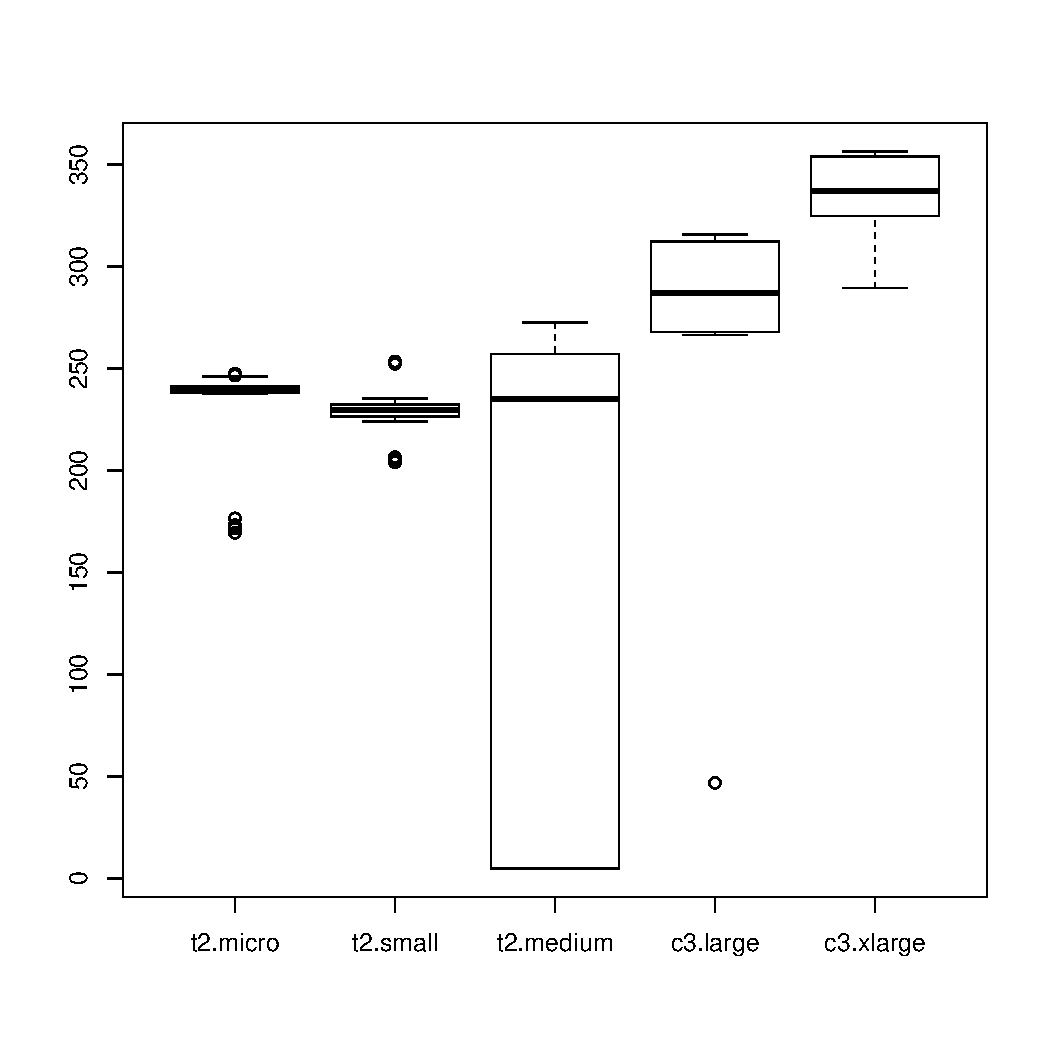
\includegraphics[width=0.5\textwidth]{plots/dbench2.pdf}
\caption{Difference between instances in Disk performances}
\label{fig:dbench2}
\end{figure}

As highlighted in Figure \ref{fig:dbench2}, the minimum time needed for the instance \textit{t2.micro} is 169.404 MB/s, whereas the maximum is 247.495 MB/s. 204.038 MB/s is the minimum and 253.5 MB/s is the maximum for the instance \textit{t2.small}, \textit{t2.medium} provides as minimum value 4.97754 MB/s and 272.515 MB/s as maximum value, the minimum time needed for the instance \textit{c3.large} is 46.8487 MB/s and the maximum is 315.7 MB/s. The minimum for the instance \textit{c3.xlarge} is 289.411 MB/s and the maximum is 356.324 MB/s.

As provided by Figure \ref{fig:dbench2}, the order of instances by the median of the disk performance from the lowest performance to highest one is as follow: \textit{t2.micro, t2.small, t2.medium, c3.large, and c3.xlarge}.

\textbf{Discussion.} The main differences between the instances \textit{t2.micro} and \textit{t2.small} are the tests \textit{Find}, which consists of finding a file in the disk. Where the second important difference we have found is the test \textit{ReadX} related to the read file operations. Moreover, the important difference between \textit{t2.small} and \textit{t2.medium} is \textit{Flush} test, which is a test related to the file operations. The same difference between \textit{t2.medium} and \textit{c3.large}. The main differences between \textit{c3.xlarge} and \textit{c3.large} are \textit{ReadX} and \textit{WriteX}, which are related to read/write on a file.


We analyzed the \textit{t2.median} data results to understand the important difference between the minimun and the maximum value provided by the instance \textit{t2.median}, as highlighted in Figure \ref{fig:dbench2}. We observe that the first two tests provide a high results, where the three other ones provide a low performance. For example, from the five instances we analyzed for \textit{t2.median}, the two performances test results provide respectively 272.515 and 271.193 MB/s, where the three other tests provide respectively 4.98222, 4.99306, and 5.0212. The same differences between for the four \textit{t2.medium} instances. We can explain that by the fact that the performance is degraded across the execution of tests, more we execute tests on the machine, the performance decreases. Hence, the instance \textit{t2.medium} loses its performance under pressure.  

\

\noindent\fbox{%
    \parbox{8.5cm}{
	\textit{\newline
	The best instance providing the best disk performances is \textit{c3.xlarge}, while the lowest performance value is provided by the instances  \textit{t2.micro} and \textit{t2.small}.
\newline
	} 
    } \par
}

\

\

\subsection{Network Throughput performances}


\textbf{Results. The averages of the throughput performances results for each instance are: 34125.6032 for the instance \textit{t2.micro}, 32274.9292 for the instance \textit{t2.small}, 43254.6048 for the instance \textit{t2.medium}, 30055.9284 for the instance \textit{c3.large}, and 42955.2664 for the instance \textit{c3.xlarge}}.


As highlighted in Figure \ref{fig:netperf}, the minimum throughput for the instance \textit{t2.micro} is 32342.23 MB/s, whereas the maximum is 37792.86 MB/s. 28951.68 MB/s is the minimum and 35593.7 MB/s is the maximum for the instance \textit{t2.small}, \textit{t2.medium} provides as minimum value 41971.34 MB/s and 45802.88 MB/s as maximum value, the minimum speed for the instance \textit{c3.large} is 29365.97 MB/s and the maximum is 30693.28 MB/s. The minimum for the instance \textit{c3.xlarge} is 30394.5 MB/s and the maximum is 48512.07 MB/s.



\begin{figure}
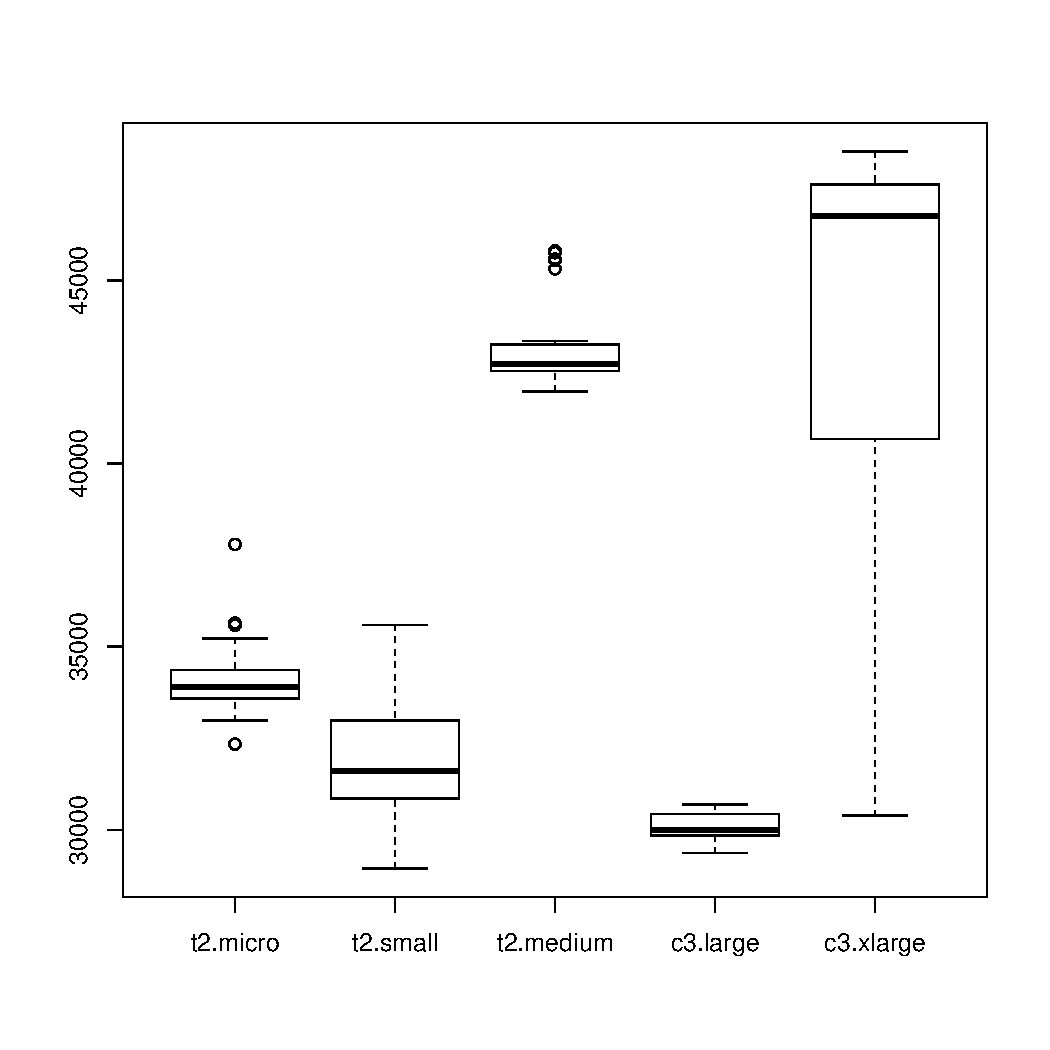
\includegraphics[width=0.5\textwidth]{plots/netperf.pdf}
\caption{Difference between instances in Network Throughput performances}
\label{fig:netperf}
\end{figure}

As provided by Figure \ref{fig:netperf}, the order of the instances studied by the median of the throughput performance is as follow: \textit{c3.large, t2.small, t2.micro, t2.medium, and c3.xlarge}.


\

\noindent\fbox{%
    \parbox{8.5cm}{
	\textit{\newline
	The best instance providing the best throughput network performances is \textit{c3.xlarge}, while the lowest performance value is provided by the instance \textit{c3.large}.
\newline
	} 
    } \par
}

\

\
\nocite{*}

\section{Discussion}
\label{sec:discussion}

\textit{t2.micro} provides the lowest performances except for throughput performances. It could be used in for a simple application that don't need any important performances. However, it provides an acceptable network throughput, which is higher than the instance \textit{t2.medium} and \textit{c3.large}.

The performance of the instance \textit{t2.small} is more important than the performance of the instance \textit{t2.micro}, except for network throughput and disk performances. 

\textit{t2.medium} takes the third importance in IO, IOPS, and disk performances, and the second place for network throughput and CPU performances.

\textit{c3.large} has good performances except network throughput. 

\textit{c3.xlarge} is the best instance in all the performances. However, it has approximately the same IOPS performances as the instance \textit{c3.large}.

The best instance to deploy software applications needing CPU performances, the best instance is \textit{c3.xlarge}, and \textit{t2.medium} comes in the second level. Moreover, the best instance that could be used by software applications that need IO performances is \textit{c3.xlarge}, while the other instances have the same low performances. Furthermore, \textit{c3.large} and \textit{c3.xlarge} can be used for the software applications needing a good IOPS performances. The instance \textit{c3.xlarge} is the more recommend instance for the application having many operations in disk. For the applications using more network could use at the first choice \textit{c3.xlarge} and at the second one \textit{t2.medium}.


\section{Conclusion}
\label{sec:conclusion}
Cloud computing involves deploying groups of remote servers and software networks that allow centralized data storage and online access to computer services or resources. In this project, we have launched five different distances and then analyzed based on five defined benchmarks. Results showed their performances in different types. C3.xlarge has better performance among all categories except network throughput, while t2.micro almost has a same low performance.

\balance
\bibliographystyle{IEEEtran}
\bibliography{assignment.bib}


\end{document}
